\subsubsection{本走行・実験走行で見つかった課題}
\paragraph{コストへのロボットの乗り上げにより動作不能になる問題}
むぎまるチームのリタイアの原因は、navigation2が経路生成をする際に参照する
コストマップにおいて、ロボットがコストに乗り上げてしまったことである。
この状況をRvizを用いて可視化した際の画像を図\label{fig:mugimaru_result}に示す。
図中のピンク色の範囲は走行不可能領域のコスト、
水色の範囲はロボットの内接円半径を考慮した走行不可能領域のコストを表している。
つまり、ロボットの中心が水色の範囲に侵入すると
ロボットが走行不可能領域にいると判断される。
図\label{fig:mugimaru_result}からロボットの中心は
水色の範囲に侵入していることが確認できる。
この状態になると、navigation2は目的地までの経路及び動作を生成しなくなる。
この状態になった後、ロボットはリカバリー動作を実行したが、
それも有効に働かずナビゲーションを中断してしまった。

この問題への対策として、走行可能領域に入るまで
安全に配慮しながら動き回るというリカバリー動作を実装することが
一つ挙げられる。
図からロボットの前方には走行可能領域があることが確認できる。
その場所まで3D LiDARにより周囲の安全を確認しながら移動可能であれば、
この問題が発生した場合にでもナビゲーションを続行できるようになると考える。
\begin{figure}[h]
  \centering
  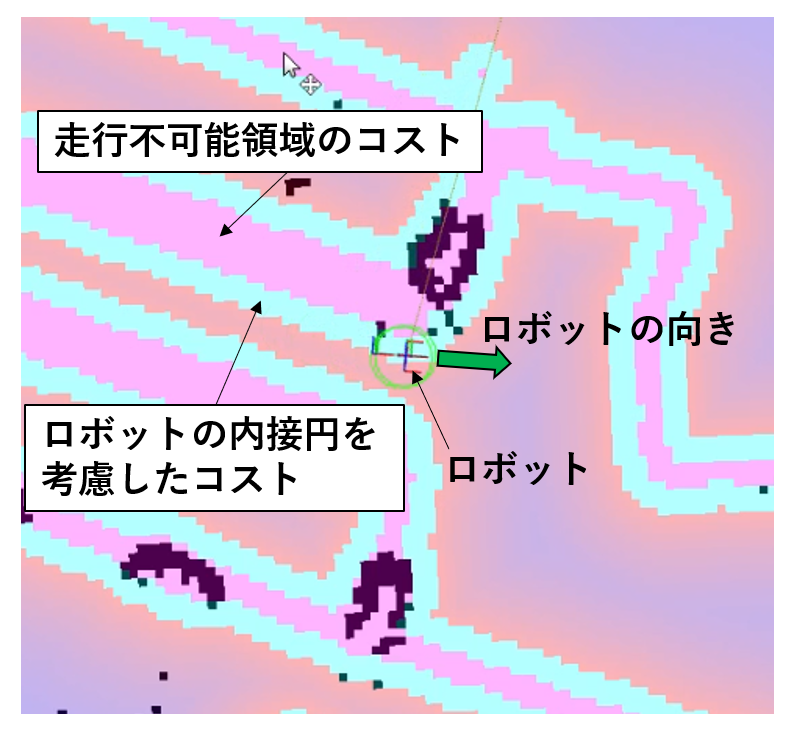
\includegraphics[width=0.9\linewidth]{figs/mugimaru_result.eps}
  \label{fig:mugimaru_result}
  \caption{ロボットがコストマップに乗り上げた状況の図} 
\end{figure}

